% vim: spell spelllang=en_gb
\documentclass[a4paper, 12pt]{article}
\usepackage[toc,page]{appendix} 
% For hyperlinks
\usepackage{hyperref}

 \hypersetup{
    colorlinks=true,
    linkcolor=blue,
    citecolor=black,        % color of links to bibliography
    filecolor=magenta,      
    urlcolor=blue,
}
\usepackage[printonlyused,withpage]{acronym}
\usepackage{geometry}
\usepackage{scrlayer} % Needed for left blank page
\emergencystretch=1em % Resolves bibliography overflow

\DeclareNewLayer[
    foreground,
    %textarea,% use only the textarea
    contents={%
      \parbox[b][\layerheight][c]{\layerwidth}
        {\centering  This page intentionally left blank.}%
    }
  ]{blankpage.fg}
\DeclarePageStyleByLayers{blank}{blankpage.fg}

 \geometry{
 a4paper,
 left=1in,
 right=1in, 
 top=1.44in,
 bottom=1.44in
 }

\usepackage{biblatex}
\addbibresource{bibliography.bib}
 
\begin{document}
 \pagenumbering{roman}

\thispagestyle{empty}
\section*{Title page}

\textsc{\large Thesis title }

\textsc{\large Yaser Kaddoura}

Note: When reviewer/examiner decides that the report is close to be finished,
contact coordinator for a report number and instructions to produce a title and
abstract page.

\newpage\null\thispagestyle{blank}\newpage

\thispagestyle{empty}
% vim; spell spelllang=en_gb
\section*{Abstract}

The more established information about a disaster, the more efficiently the disaster management is
done by the concerned parties to handle the situation. People tend to share their experiences during
disastrous events using social media, making them potential data sources. This thesis project
implements a pipeline to extract knowledge from Twitter about flood events. It determines
flood-relevant tweets using a classifier and identifies geographical locations mentioned in the
tweets using a hybrid geoparsing approach. At the end of the pipeline, the spatial, temporal, and
textual aspects of the results are presented using an interactive visual interface. The implemented
pipeline is exemplified using historical tweets created during past flood events.



\newpage\null\thispagestyle{blank}\newpage

\tableofcontents

\newpage

\listoffigures

\newpage

\listoftables
\newpage

% vim: spell spelllang=en_gb
\section*{List of Acronyms}

\begin{acronym} 
 \acro{ML}{Machine Learning}
 \acro{NER}{Named-entity recognition}
\end{acronym}



\newpage
\newpage\null(Might be needed to make introduction starts at odd page number)
\thispagestyle{blank}\newpage


\pagenumbering{arabic}

\section{Introduction}

Some text \ac{ML}

Dummy citation~\cite{barkerDevelopmentNationalscaleRealtime2019}

 \begin{figure}[ht]
    \centering
    \caption{Dummy figure} 
\end{figure}

\begin{table}[h!]
\centering
\begin{tabular}{||c c c c||} 
 \hline
 Col1 & Col2 & Col2 & Col3 \\ [0.5ex] 
 \hline\hline
 1 & 6 & 87837 & 787 \\ 
 2 & 7 & 78 & 5415 \\
 3 & 545 & 778 & 7507 \\
 4 & 545 & 18744 & 7560 \\
 5 & 88 & 788 & 6344 \\ [1ex] 
 \hline
\end{tabular}
\caption{Dummy table}
\end{table}


\newpage

\printbibliography[heading=bibintoc, title={References}]

\newpage

\section{Draft}

 \begingroup\makeatletter\def\@currenvir{verbatim}
\verbatim
*** Abstract
Write abstract last
- What did you do?
  - Extract context from tweets regarding floods
- Why did you do it? What question were you trying to answer?
  - Floods has negative impact
- How did you do it? State methods.
  - Identify tweets that talks about floods
  - Identify locations
  - Visualize the output
- What did you learn? State major results.
- Why does it matter? Point out at least one significant implication
  - Helps for disaster management
  - flood detection specific for swedish lang/sweden
*** Introduction
A monitoring system Using streaming API provided by twitter, a
- How usage of social media can solve the problem
  - Integration with SMHI
  - Forcasting
  - Mention voulenteered geographic information VGI
  - Early detection
  - During disaster management (helping in need)
  - Post disaster analysis (assessing the damage)
  - [[https://www.physio-pedia.com/Disaster_Management][Disaster Management - Physiopedia]] (Disaster management)
- What to expect in thesis (Problems tackled)
  - focus on floods in Sweden
  - Extracting historical tweets that are flood related
  - extracting locations
  - Visualize the output
  - The pipeline is verified on some past flood events
- [[https://en.wikipedia.org/wiki/Early_warning_system][Early warning system - Wikipedia]]
- [[https://en.wikipedia.org/wiki/Disaster_response][Disaster response - Wikipedia]]
- [[https://en.wikipedia.org/wiki/Emergency_management#Preparedness][Emergency management - Wikipedia]]
- [[https://www.climatechangepost.com/sweden/river-floods/][River floods - Sweden - Climatechangepost.com]]
*** Literature review
- Introduction
- Data collection
  - labeled, unlabaled, autolabeling (page 8 of [cite:@petersenIdentificationExplorationExtreme2021])
  - Using twitter api, streaming, 3rd party, images
  - Keywords used (multinlingual)
  - Data processing
    - spam, filtering
- Location specific or global
  - global, local
  - methods
    - markov chains using data from user profile and historical tweets
  - twitter info (geotag, entities, etc.)
  - 1% of tweets are geotaged    [cite:@middletonRealTimeCrisisMapping2014]
- Flood detection
  - transformers
  - CNN
  - word embeding
  - Mention the progression from using basic classifiers to transformers
- Data visualization
- What problems they address
  - Early detection of events via monitiring a stream
  - Disaster management [[https://12ft.io/proxy?q=https://www.physio-pedia.com/Disaster_Management][12ft | Disaster Management - Physiopedia]]
- Maybe evaluate other works
- The location of my solution in the context of the existing literature
*** Methods
- git repo and major libraries used and for what purpose
- reason for picking each method
- packages used in each step
- how to replicate (Refer to README in git repo)
**** Data collection
- Preprocessing
  - Text
  - Tweets
  - Maybe, mention reprocessing in different sections, since each one's 
  preprocessing can be different
  - Swedish only, translated to english for classification
- Data sources
  - Twitter API
    - query used
    - major parameters extracted
    - Used for verification an use cases
  - manually annotated Swedish
    - features
    - Available columns
    - amount
    - Training dataset doesn't explicit mention the location,
    - percentage of labeled relevant (is it imbalanced?)
    - language
- Spams
  - why they are bad
  - Reasons for spam
  - How to handle them
**** Flood classification
- Transformers - Self-attention - took the world of NLP by a storm - 
Can be used for other tasks Their need for big dataset - 
Pretrained models that can be fine tuned with smaller datasets to
improve their performance for a more specific task.
Summary of architecture
overthrowing RNN from its throne by a long shot making itself even feasible 
for other tasks
More performant (parallize)
RNN attention and its capabilities

HuggingFace is a framework that provides a unified API for over more than 
50 architectures making it
easier for users to integrate NLP models into their applications.
Supports TensorFlow and PyTorch
It's model hub Contains tens of thousands of pretrained models
Ease of access to the state-of-the-art pretrained model
Has a big amount of datasets.

DistilBERT.1 The main advantage of this model is that it achieves comparable 
performance to BERT,
while being significantly smaller than BERT while being significantly smaller and 
more efficient. 
This enables us to train a classifier in a few minutes.
Use swedish directly or translate it then use english transformer. Given that 
the best transformers use english and that
the existence of English labeled datasets, it's more advantageous to translate it.
**** Location extraction
- Talk about Toponym recognition & Toponym resolution
- Usage of NER & gazetteer (Mention packages)
- Extract Swedish locations and one location if more than one two is given in 
one tweet (smallest area)
- Mention that geo-referencing isn't viable since users barely use it 
(Show reference)
**** Visualization
- Requirements
- Purposes
- What's the difference between this section and the one in Results?
  - Should I discuss the plots here and mention how they fulfill their roles in 
  results section?
- Discuss every plot
- Discuss their interactivety
- Mention any significant logic that's being done under the hood
*** Results
- Introductory section
- Flood classification training ::
  eval_accuracy   eval_f1   eval_precision   eval_recall
  0.95885   0.93506            0.93506       0.93506
- Location extraction
  - What types of locations are being extracted
- Visualization
- Verification (Use cases)
  - Talk about the pipeline (Tweets extracted during a time interval of one week 
  after the flood event)
  - Mention the query and package used
*** Discussion
- Mention briefly that the pipeline successfully identified the concerned 
flood event by using the
  results as evidence
- How reliable the methods are
  - Classification
- Discuss results
  - Locations
    - How many locations are extracted for that concerned location
    - Comparison between extracted locations and the manually annotated dataset
    - Same keyword can refer to more than one location
- Verification
  - Does the results seem reliable?
  - Maybe make a comparison between two flooding events
  - How accurate each part of the pipeline
    - Are the classified tweets reasonable?
    - Are the extracted locations mention the concerned flood event
    - Show screenshots of the plots while discussing points
    - Does the accuracy differ among the use cases
*** Further works
- Streaming for live event detection
- Identifying flood events explicitly
- Include other types of data images to the pipeline
- Include other sources of data such as GDELT, other social media for training 
and analysis Handling noise (spammers)
- Increase accuracy for different parts of the pipeline
- Use pipeline for other locations and topics by updating a part of the pipeline 
(e.g. twitter API query, text pre-processing for different languages)
- Using other languages
- Visualization improvements
- Augment warning systems pipeline by including this approach
- Text analysis for assessing damages (If topic modeling isn't used in main project)
*** Conclusion
- How the results show that this medium has potential to assist in the problems
- List some practical uses the solution gives for disaster management
- Making a grand scale system for anything based on different sources social media 
and other resources.
  - Challenges that could be faced
- Emphasis that the problem (disasters) won't disappear and they will only become 
worse in the future and that making use of solutions augmenting the coping for them.
\end{verbatim}

% vim: spell spelllang=en_gb
\appendix
\chapter{Diagrams}\label{appendix:raw}
\begin{figure}
\begin{center}
  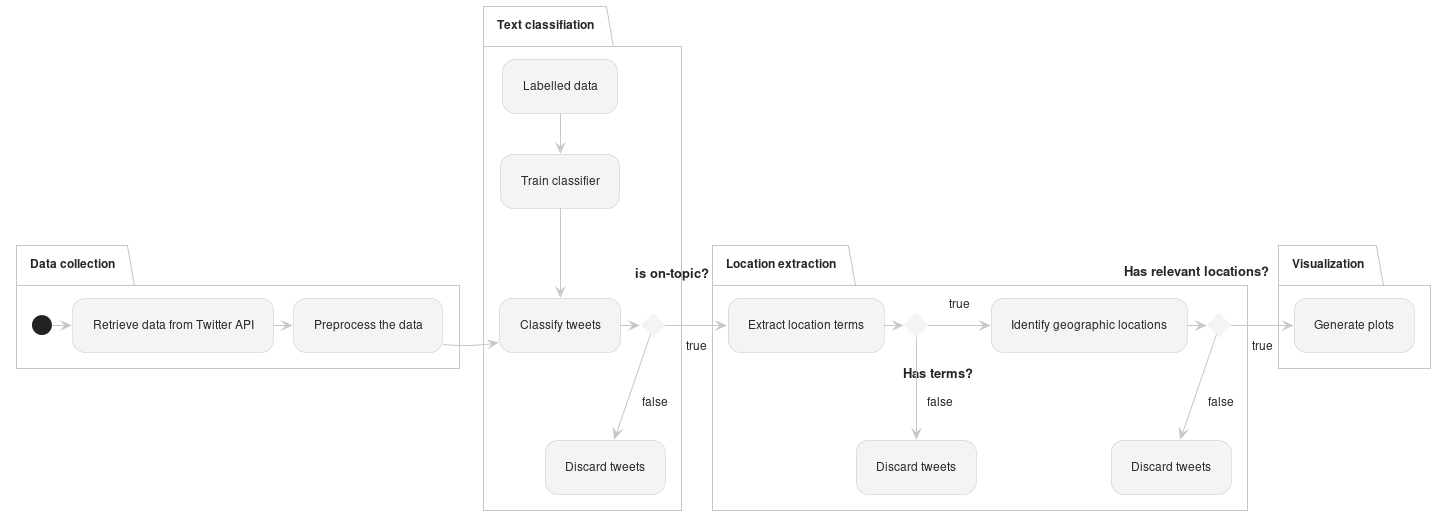
\includegraphics[angle=90, width=\dimexpr\textwidth-11cm\relax, height=\textheight, keepaspectratio]{./images/pipeline.png}
\end{center}
\caption{Flow chart for the pipeline}
\label{fig:flow_chart_big}
\end{figure}

\chapter{Examples}\label{appendix:examples}
\section{Nominatim output example}
 \begin{verbatim}
  {
    "place_id": "100149",
    "licence": "Data © OpenStreetMap contributors, 
                ODbL 1.0. https://osm.org/copyright",
    "osm_type": "node",
    "osm_id": "107775",
    "boundingbox": ["51.3473219", "51.6673219", 
                    "-0.2876474", "0.0323526"],
    "lat": "51.5073219",
    "lon": "-0.1276474",
    "display_name": "London, Greater London, England, 
                     SW1A 2DU, United Kingdom",
    "class": "place",
    "type": "city",
    "importance": 0.9654895765402,
    "icon": "https://nominatim.openstreetmap.org/
             images/mapicons/poi_place_city.p.20.png",
    "address": {
      "city": "London",
      "state_district": "Greater London",
      "state": "England",
      "ISO3166-2-lvl4": "GB-ENG",
      "postcode": "SW1A 2DU",
      "country": "United Kingdom",
      "country_code": "gb"
    },
    "extratags": {
      "capital": "yes",
      "website": "http://www.london.gov.uk",
      "wikidata": "Q84",
      "wikipedia": "en:London",
      "population": "8416535"
    }
  }                           
  \end{verbatim}
                


\end{document}
